\documentclass[tikz,border=10pt]{standalone}
\usepackage{tikz}
\usetikzlibrary{arrows.meta, decorations.pathmorphing, positioning}

\begin{document}
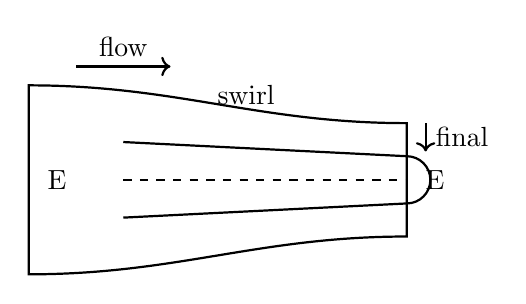
\begin{tikzpicture}[scale=1.2]

% Outer duct shape
\draw[thick] (0,1) to[out=0,in=180] (4,0.6) -- (4,-0.6) to[out=180,in=0] (0,-1) -- cycle;

% Inner pipe
\draw[thick] (1,0.4) -- (4,0.25);
\draw[thick] (1,-0.4) -- (4,-0.25);
\draw[thick] (4,0.25) arc[start angle=90,end angle=-90,radius=0.25];
\draw[thick, dashed] (1,0) -- (4,0);

% Flow arrow
\draw[->, thick] (0.5,1.2) -- (1.5,1.2) node[midway, above] {flow};

% Final pipe label
\draw[->, thick] (4.2,0.6) -- (4.2,0.3) node[midway, right] {final};

% Swirl label
\node at (2.3,0.9) {swirl};

% "E" labels at entrance and exit
\node at (0.3,0) {E};
\node at (4.3,0) {E};

\end{tikzpicture}
\end{document}